\newpage
\section{Preparación de datos}
\subsection{Enunciado}
Estandarización: Antes de aplicar PCA, asegúrate de estandarizar las variables cuantitativas para que tengan media cero y desviación estándar uno. Esto es importante, ya que PCA es sensible a la escala de los datos. Nota: Sklearn utiliza la matriz de covarianza y esa es la razón por la que hay que estandarizar previamente. 

Matriz de Correlación: Visualizar la matriz de correlación de las variables originales antes de aplicar PCA. Como regla general:
Un rango óptimo de correlación entre variables se sitúa entre ±0.5 y ±0.9. Las correlaciones más bajas indican que las variables no están relacionadas, lo que podría implicar que PCA no reducirá significativamente la dimensionalidad. Si la correlación entre muchas variables es cercana a cero, PCA puede no ser tan efectivo. Idealmente, deberías observar varias correlaciones moderadas a fuertes entre las variables.

\subsection{Estandarización de datos}
Tomando en cuenta las variables que se utilizarán, esto nos muestra la transformación utilizando Sklearn para el escalado de la misma.

\begin{table}[H]
\centering
\begin{tabular}{|l|r|}
\hline
\textbf{Variable} & \textbf{Media} \\ \hline
Age                       & -3.504377e-17 \\ \hline
JobLevel                  & -2.658493e-17 \\ \hline
MonthlyIncome             & -4.471102e-17 \\ \hline
NumCompaniesWorked         &  1.450087e-17 \\ \hline
TotalWorkingYears          & -1.208406e-18 \\ \hline
YearsAtCompany             & -3.021015e-17 \\ \hline
YearsInCurrentRole         &  9.063045e-17 \\ \hline
YearsSinceLastPromotion    &  1.208406e-18 \\ \hline
YearsWithCurrManager      & -2.779334e-17 \\ \hline
\end{tabular}
\caption{Media de cada variable estandarizada}
\end{table}

\textbf{Observación:}
Podemos evidenciar en el siguiente cuadro que la media está 
cerca de 0 (por ejemplo, entre -1e-17 y 1e-18).

\begin{table}[H]
\centering
\begin{tabular}{|l|r|}
\hline
\textbf{Variable} & \textbf{Desviación Estándar} \\ \hline
Age                        & 1.00034 \\ \hline
JobLevel                   & 1.00034 \\ \hline
MonthlyIncome              & 1.00034 \\ \hline
NumCompaniesWorked         & 1.00034 \\ \hline
TotalWorkingYears          & 1.00034 \\ \hline
YearsAtCompany             & 1.00034 \\ \hline
YearsInCurrentRole         & 1.00034 \\ \hline
YearsSinceLastPromotion    & 1.00034 \\ \hline
YearsWithCurrManager       & 1.00034 \\ \hline
\end{tabular}
\caption{Desviación estándar de cada variable estandarizada}
\end{table}

\subsection{Matriz de correlación}
Utilizando los datos estandarizados, se procede a calcular la matriz de correlación.

\begin{figure}[h!]
    \centering
    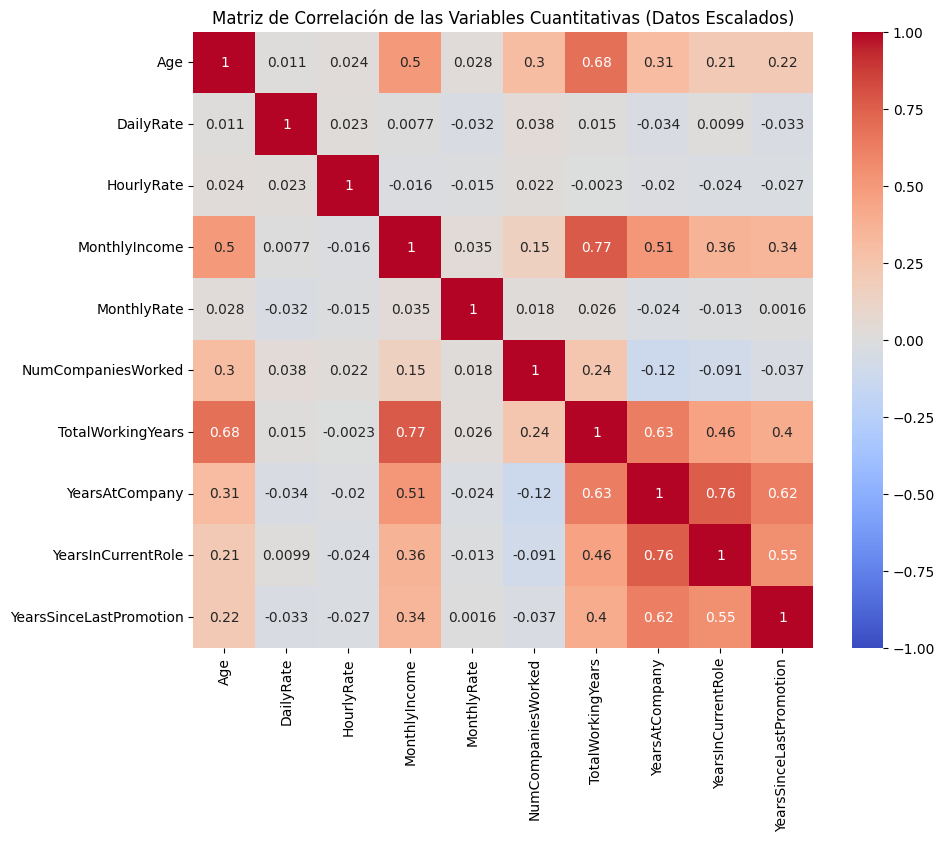
\includegraphics[width=1\textwidth]{images/matriz-de-correlacion.png}
    \caption{Matriz de correlación de las variables cuantitativas}
    \label{fig:matriz_correlacion}
\end{figure}

Podemos observar que la matriz de correlación es una matriz simétrica, 
con valores en la diagonal principal iguales a 1, aunque vemos que la variable NumCompaniesWorked 
tienen una correlación cercana a 0 lo que indica no hay una relación lineal fuerte entre 
esa una variable y las otras en la matriz.